\section{Standard parameters for the runs}
%
In this thesis, we have chosen the following shape of the source
%
\begin{align*}
    S = AH(\rho,s_{\text{profile}},c_{\text{profile}},w_{\text{profile}})
\end{align*}
%
where $H$ is defined in \cref{eq:hat}, and $A$ is an amplitude chosen so that the maximum of the normalized $n$ is around $1$.
Note that the source is uniform in along the parallel direction.
A more probable scenario would probably be that the source would decrease along the parallel direction, until it is increased around the SE due to recycling from the wall.
In any case, finding the proper shape of the source seems to be challenging, and is probably only accurate if detailed atomic physics is taken into account.
Although interesting and relevant, such atomic processes is outside the scope of this thesis.
If nothing else is mentioned, the standard input for the simulations done are given in \cref{tb:grid,tb:input,tb:source}.
%

\begin{table}[!htb]
    \begin{minipage}{.3\linewidth}
      \centering
      \caption{Grid size used for the simulations.}
        \colorme
        \begin{tabular}{c|ll}
        \hline\hline
        %
        Variable & Value \\
        %
        \hline
        %
        $n_\rho$   & $32$  \\
        $n_z$      & $66$  \\
        $n_\theta$ & $256$ \\
        \hline\hline
        \end{tabular}
        \label{tb:grid}
    \end{minipage}%
    \hfill
    \begin{minipage}{.3\linewidth}
      \centering
        \caption{Standard parameters used in the simulations.}
            \colorme
            \begin{tabular}{c|ll}
            \hline\hline
            %
            Variable & Value & Units\\
            %
            $L_\rho$  & $0.0$            & $\m$     \\
            $L_z$     & $2.80$           & $ \m$    \\
            $n_0$     & $1\cdot 10^{19}$ & $\m^{-3}$\\
            $T_{e,0}$ & $2.5$            & $\eV$    \\
            $B_0$     & $0.1$            & $\T$     \\
            $n_n$     & $0.0$            & $\m^{-3}$\\
            Gas       & Ar               &          \\
            \hline\hline
            \end{tabular}
            \label{tb:input}
    \end{minipage}
    \hfill
    \begin{minipage}{.3\linewidth}
      \centering
        \caption{Source parameters used in the simulations.}
            \colorme
            \begin{tabular}{c|ll}
            \hline\hline
            %
            Variable & Value \\
            %
            \hline
            $s_{\text{profile}}$ & $5/L_\rho$\\
            $c_{\text{profile}}$ & $0$       \\
            $w_{\text{profile}}$ & $L_\rho$  \\
            \hline\hline
            \end{tabular}
            \label{tb:source}
    \end{minipage}
\end{table}
%
Input parameters from the implementation is found in the tables in \cref{chap:implBOUT++,chap:additionalImplementation}.

\section{Running the simulations}
\label{sec:initRun}
%
From the following initial conditions of the normalized evolved quantities%
%
\footnote{$\Om$ is used rather than $\Om^D$ when simulating using the Boussinesq approximation}%
%
\begin{align*}
    \ln(n)    =& 0\\
    j_\|      =& 0\\
    nu_{i,\|} =& \frac{z}{L_z}\\
    \Om^D     =& 0
\end{align*}
%
the simulations are performed in three following steps
%
\begin{enumerate}[noitemsep]
    \item The simulation is allowed to evolve freely to a steady state condition (that is, when there is a minimal difference between the time steps) using only one point in $\theta$.
        Usually this takes around $4000t\om_{ci}$.
    \item The simulation is expanded to $n_\theta = 256$, and run for additional $50t\om_{ci}$ in order to ensure that the system is still in a steady state.
    \item A perturbation in the form of white noise with an amplitude of $1\cdot10^{-6}$ is added to $\Om^D$%
        \footnote{Different approaches has been used for the perturbation.
            It should be noted that some of these gives a different route to the turbulent state (i.e. some perturbations dies out, while others have some intermediate non-linear steps before the linear growth rates), but gives (with very little difference) the same growth rates and the same statistical behavior of the saturated turbulence as the perturbation method stated.}%
        %
    \item If the system is unstable to small perturbations, and if there are no "crashes" in the simulation, a saturated turbulence state is eventually reached.
\end{enumerate}
%
All the simulations presented here are run on the \texttt{A1} (Broadwell) partition of the \texttt{Marconi} super cluster located at CINECA at Casalecchio di Reno (Bologna).
At the time of writing the cluster operated with the following specifications \cite{Marconi2016Web}
%
\begin{enumerate}[noitemsep]
    \item Model: Lenovo NeXtScale
    \item Architecture: Intel OmniPath Cluster
    \item Nodes: $1512$
    \item Processors: $2\times18$-cores Intel Xeon E$5-2697$ v$4$ (Broadwell) at $2.30$ GHz
    \item Cores: $36$ cores/node, $54432$ cores in total
    \item RAM: $128$ GB/node, $3.5$ GB/core
    \item Internal Network: Intel OmniPath Architecture $2$:$1$
    \item Disk Space: $17$PB (raw) of local storage
    \item Peak Performance: $2$ PFlop/s
\end{enumerate}
%
For each simulation, $2$ nodes has been allocated using $48$ cores.
This has been found to give a good speed-up (as compared to use one node) with a good trade off between the ration of simulation time to communication time per core.

\section{Resolution}
\label{sec:resolution}
%
In order to have a properly resolved grid, we need to properly resolve the gradient length scales.
To save computational time, a small number of grid points is preferable.
If we assume that the maximum gradient length scale from the model is around $\rho_s$, we should have $\frac{n_\rho}{L_\rho/\rho_s}>1$.
However, we have in this work found that $\frac{n_\rho}{L_\rho/\rho_s}\approx1$ can give simulation crashes, so a radial resolution of $\frac{n_\rho}{L_\rho/\rho_s}\approx3$ is aimed.
The same argument goes for the poloidal direction, where $L_\theta=2\pi L_\rho$.

As mentioned in \cref{chap:drift-order} the resolution in the parallel direction can be less since longer gradient scale lengths are found in the parallel direction as a consequence of the separation of scales.
The sheath sets the gradient scale length in the parallel direction, as will be explained in \cref{sec:parProf}.
Despite that the gradient scale sets a lower constraint on $n_z$, a see-sawing pattern is observed in simulations with a flow towards an end-plate for low $n_z$.
This problem has been observed in other plasma fluid codes dealing with sheath boundaries, but has to the authors best knowledge not been published.
For the work presented here, the problem is encountered for $j_\|$ as is illustrated in \cref{fig:see-saw}%
\footnote{It should be noted that running the simulations with odd number of points show similar behavior to what is presented in \cref{fig:see-saw}.}%
%
.
%
\begin{figure}[htb]
    \centering
    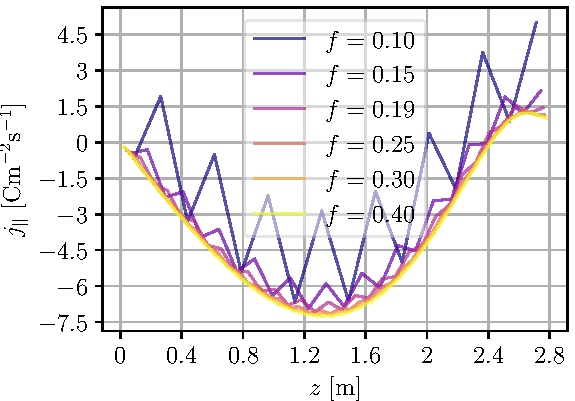
\includegraphics{fig/results/jParRipple006}
    \caption{See-saw oscillations for $B=0.06\T$ in the steady-state using $16, 24, 32, 42, 50$ and $66$ grid points in the parallel direction.
        $f$ is defined in \cref{eq:defF}
    }
    \label{fig:see-saw}
\end{figure}
%

\noindent
To get a better understanding of this behavior, the different terms in \cref{eq:celma_j_par} in the steady-state has been plotted in \cref{fig:jParBalance}.
%
\begin{figure}[htb]
    \centering
    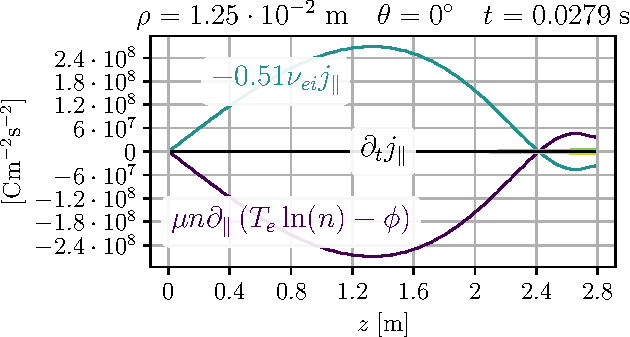
\includegraphics{fig/results/jParBalanceNy66}
    \caption{The different terms making up \cref{eq:celma_j_par} in the steady-state for $n_z=66$ for $B=0.06$.
    }
    \label{fig:jParBalance}
\end{figure}
%
It is clear that the steady state is dominated by a balance between the Boltzmann response of the electrons and resistive terms.
This is also seen for lower $n_z$, albeit with stronger oscillations in the Boltzmann response and the resistive term for decreasing $n_z$.
As the resistive term is $\propto j_\|$ it cannot be the cause of the observed see-sawing.
Thus we can conclude that the see-sawing behavior comes from the difference between the logarithm of the density and the potential.

One could imagine that the see-sawing came from catastrophic cancellation between $\ln(n)$ and $\phi$.
If this was the case, the see-sawing would be even worse for an increased mass ratio $\mu$.
In fact, the opposite behavior is observed.
Running the simulations with $\text{H}$ gives more see-sawing than $\text{Ar}$.
The explanation can be found by looking at the fraction $f$ defined by
%
\begin{align}
    f \defined \frac{n_z}{L_z/\rho_s},
    \label{fig:defF}
\end{align}
%
which describes the resolution in terms of $\rho_s$.
We can now observe that
%
\begin{align*}
  f = \frac{n_zc_s}{L_z \om_{ci}}
    = \frac{n_z\sqrt{T_e}m_i}{\sqrt{m_i} L_z ZeB}
    = \frac{n_z\sqrt{T_em_i}}{L_z ZeB},
\end{align*}
%
i. e. it is proportional with $m_i$.
On this argument, running simulations with singly ionized $\text{Ar}$ gives a better resolution of $\sqrt{m_{\text{Ar}}/m_H}\approx6.3$ as compared with $\text{H}$.
That increased oscillations has been observed with simulations done with increasing $B$ and $L_z$ strengthens the hypothesis as $f\propto 1/BL_z$.

To keep the oscillations at a minimum, we require $f > 0.2$ in the simulations performed here, which sets a lower bound on $n_z$
Ideally, we would like to reduce the number of parallel points to speed up the simulations.
Therefore some alternative strategies to lower the grid-size oscillation is discussed in the following.

Increased artificial viscosity will alleviate the problem.
Unfortunately, it is found that the artificial viscosity coefficients needed for a smooth $j_\|$ makes the artificial viscosity term dominate, such that the steady state is defined by a balance between the Boltzmann terms, the resistive term and the artificial terms.
The same holds true if the artificial viscous terms are changed with hyperviscous terms of order $4$ (i.e. with $\partial_z^4$ terms).

To reformulate the problem into a finite volume problem seems to be a good idea as fluxes through the cell centers are conserved.
However, the same grid-size oscillation problem has been found in finite volume models \cite{Dudson2017Private}.

Finally, a split-scheme could lessen the problem.
Since the discretization of $n\mu\partial_z\L(\ln(n)-\phi\R)$ is done with a centered FD scheme, odd and even grid points will be decoupled.
That is, $\partial_z\L(\ln(n)-\phi\R)$ for odd grid points will only depend on the even points and vice versa.
For advective terms references \cite{Honein2004,Pirozzoli2011} suggest a skew-symmetric split in the form $\div\L(a\ve{u}\R) = \frac{1}{2}\L[\div\L(a\ve{u}\R) + a\div\ve{u} + \ve{u}\cdot\grad a\R]$ where all the right hand terms are discretized using centred difference schemes to get rid of the decoupling.
Although arising from a divergence term, rewriting $n\mu\partial_z\L(\ln(n)-\phi\R)$ to $\partial_z\L(n\mu\L[\ln(n)-\phi\R]\R)-\L(\ln(n)-\phi\R)\partial_z\L(n\mu\R)$ may help for the grid-size oscillations.
This has, however, not been tried in the work presented in this thesis.
